\documentclass[english,xcolor=x11names]{beamer}
\usepackage[utf8]{inputenc}
\usepackage[T1]{fontenc}
\usepackage{babel}
\usepackage{graphicx}
\usepackage{tikz}
\usepackage{pgfplots}
\usepackage{hyperref}
\usepackage{libertine}
\usepackage{eulervm}
\usepackage[ttdefault]{sourcecodepro}
\usepackage[fixed]{fontawesome5} 
\usepackage{relsize}
\usepackage{amsmath}
\usepackage{amssymb}
\usepackage{bm}
\usepackage[autostyle=true]{csquotes} 
\usepackage[backend=biber,style=authoryear,citestyle=alphabetic,maxnames=1,url=false,doi=false,isbn=false,dashed=false,mincrossrefs=1000]{biblatex}
\usepackage{apptools}
\usepackage{appendixnumberbeamer}
\usepackage{tikz}
\usepackage{listings}
\usepackage{xspace}
\usepackage{biblatex}
\usepackage{tabularx}
\usepackage{booktabs}
\usepackage{graphicx}
\usepackage{multirow}
\usepackage{arydshln}
\usepackage{xcolor}
\usepackage{colortbl}
\usepackage{transparent}

\let\tmp\mod \let\mod\bmod \let\bmod\tmp
\let\varemptyset\emptyset \let\emptyset\varnothing
\let\tmp\epsilon \let\epsilon\varepsilon \let\varepsilon\tmp
\let\tmp\phi \let\phi\varphi \let\varphi\tmp

\usetheme{boxes} % Simple
\definecolor{fsublue}{RGB}{0,47,93}
\setbeamercolor{structure}{fg=fsublue}
\usefonttheme[onlymath]{serif}
\setbeamerfont{title}{series=\bfseries,parent=structure}
\setbeamersize{description width=2em}
\setbeamersize{text margin left=0.5cm, text margin right=0.5cm}
\setbeamercovered{transparent}
\setbeamertemplate{frametitle continuation}[from second][\usebeamercolor{normal text}\color{fg!40!bg}\insertcontinuationtext] 
\beamertemplatenavigationsymbolsempty
\addtobeamertemplate{navigation symbols}{}{%
	\usebeamerfont{footline}%
	\usebeamercolor[fg]{footline}%
	\quad%
	\raisebox{0.5ex}{\IfAppendix{A-}{}\insertframenumber/\inserttotalframenumber}%
	\enskip%
	\vspace{0.5ex}%
}
\defbeamertemplate{description item}{align left}{\insertdescriptionitem\hfill}
\setbeamertemplate{description item}[align left]

\newcommand{\textttsmall}[1]{\texttt{\smaller #1}}
\newcommand{\query}[1]{\textttsmall{#1}}
\newcommand{\domain}[1]{\href{http://#1}{\mbox{\textttsmall{#1}}}}

\renewcommand{\bibfont}{\smaller}
\renewcommand{\pgfuseimage}[1]{\includegraphics[scale=.65]{#1}} % Shrink book images.
\setlength{\bibhang}{0pt} % Remove hanging indent.
\AtEveryCite{\smaller\color{fg!60!bg}} % Make cites smaller, dimmed.

\pgfplotsset{
  compat=1.18
}
\definecolor{mediumgray}{gray}{0.60}
\definecolor{webiscodebasic}{rgb}{0.2,0.2,0.2}
\definecolor{webiscodekeyword}{rgb}{0.0,0.5,0.0}
\definecolor{webiscodekeywordself}{rgb}{0.7,0.4,0.6}
\definecolor{webiscodeidentifier}{rgb}{0.0,0.0,0.0}
\definecolor{webiscodecomment}{rgb}{0.25,0.5,0.5}
\definecolor{webiscodestring}{rgb}{0.75,0.12,0.12}
\definecolor{webiscodedecorator}{rgb}{0.6,0.3,0.0}
\lstdefinestyle{webisstyle}{
  basicstyle=\fontsize{6pt}{7pt}\selectfont\ttfamily\color{webiscodebasic},
  keywordstyle=\color{webiscodekeyword},
  identifierstyle=\color{webiscodeidentifier},
  commentstyle=\color{webiscodecomment},
  stringstyle=\color{webiscodestring},
  showstringspaces=false,
  frame=lines,
  framesep=0.7em,
  rulesep=0.5em,
  framerule=0.1em,
  keepspaces=true,
  tabsize=2,
  showtabs=false,
  numbers=none,
  literate=
    {->}{{\textrightarrow}}{2}
    {>=}{{\(\geq\)}}{2}
    {<=}{{\(\leq\)}}{2}
    {!=}{{\(\neq\)}}{2},
}
\lstloadlanguages{Python}
\lstset{
  style=webisstyle,
  language=Python,
  emph={[1]def,class},
  emphstyle={[1]\color{webiscodekeyword}\bfseries},
  emph={[2]self,cls},
  emphstyle={[2]\color{webiscodekeywordself}},
  emph={[3]@dataclass},
  emphstyle={[3]\color{webiscodedecorator}},
}

\newcommand{\bibliographyframe}{
\begin{frame}[t,allowframebreaks]{References}
	\begin{thebibliography}{10}
		\beamertemplatebookbibitems
		\printbibliography
	\end{thebibliography}
\end{frame}
}
\newcommand{\titleframe}{
	\begingroup
	\setbeamertemplate{navigation symbols}{}
	\frame[plain]{\titlepage}
	\endgroup
}

\newcommand{\pro}{\item[\(\bm{+}\)]} % Pro item
\newcommand{\contra}{\item[\(\bm{-}\)]} % Contra item
\newcommand{\thankyouname}{Thank you, stay tuned for more!}
\newcommand{\thankyou}{\vfill\hfill\emph{\thankyouname}}
\newcommand{\todocite}{{\smaller\color{red}[CITE]}\xspace}
\newcommand{\todo}[1]{{\smaller\color{red}[#1]}}

% Bibliography
% \addbibresource{TODO.bib}

\title{\Huge The Archive Query Log\vspace*{-2ex}}
\author{\scriptsize Heinrich \and Sebastian \and Maik \and Lukas \and Harry \and Benno \and Matthias \and Martin}
\institute{}
\date{}
\titlegraphic{\vspace*{-7ex}
\includegraphics[width=0.77\linewidth]{meme-aql}
}

\begin{document}

\titleframe

\begin{frame}{Query Logs}
  \begin{columns}
    \begin{column}{0.55\linewidth}
      \only<-2>{
        \only<2>{\vspace{0.65ex}}
        \begin{block}{What are they good for?~\faIcon{grin-wink}}
          \begin{itemize}
            \item Query understanding
            \item Learning to rank
            \item SERP analysis
          \end{itemize}
        \end{block}
        \vspace{4ex}
        \uncover<2>{
          \begin{block}{What's the issue?~\faIcon{meh}}
            \begin{itemize}
              \item Most are \textbf{private}
              \item Public ones \textbf{much smaller}
            \end{itemize}
          \end{block}
        }
        \vspace{2ex}
      }
      \only<3->{
        \begin{center}
          
\includegraphics[width=0.7\linewidth]{meme-restricted-access}
        \end{center}
      }
    \end{column}
    \uncover<2->{
      \begin{column}{0.45\linewidth}
        \begin{center}
          \vspace*{-3ex}%
          \only<1>{\vspace{1.3ex}\transparent{0.3}
\includegraphics[width=\linewidth]{wordcloud-without-aql}\\}%
          \only<2->{
\includegraphics[width=\linewidth]{wordcloud-without-aql}\\}%
          Previous Logs
          \vspace{5ex}
        \end{center}
      \end{column}
    }
  \end{columns}
\end{frame}

\begin{frame}{Web Archive to the rescue!}
  \begin{columns}
    \begin{column}{0.55\linewidth}
      \begin{block}{But how?}
        \vspace{1ex}
        \begin{enumerate}
          \item List SERP URLs from Web Archive
          \item Parse query
          \item Download SERP HTML
          \item Parse search results
        \end{enumerate}
      \end{block}
      \vspace{4ex}
      \begin{block}{Like this\textellipsis}
        \vspace{2ex}
        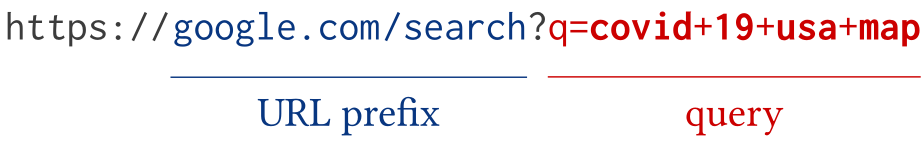
\includegraphics[width=1.1\linewidth]{url-pattern}\\
      \end{block}
    \end{column}
    \begin{column}{0.45\linewidth}
      \begin{center}
        \vspace*{-3ex}
        
\includegraphics[width=\linewidth]{wordcloud}\\
        With the AQL
        \vspace{5ex}
      \end{center}
    \end{column}
  \end{columns}
\end{frame}

\begin{frame}{Meet the \textbf{Archive Query Log}}
  \framesubtitle{%
    \scriptsize%
    \href{https://github.com/webis-de/archive-query-log}{\faIcon{github}\enskip\texttt{webis-de/archive-query-log}}
  }
  \begin{columns}[c]
    \hspace{0.3em}
    \begin{column}{0.42\linewidth}
      \begin{itemize}
        \item[\smaller\faSearch] 356 million queries
        \item[\smaller\faList] 166 million SERPs
        \item[\smaller\faFile*] 1.7 billion search results
        \item[\smaller\faCalendar*] across 25 years
        \item[\smaller\faServer] 550 search providers
      \end{itemize}
      \vspace{3ex}
    \end{column}
    \begin{column}{0.56\linewidth}
      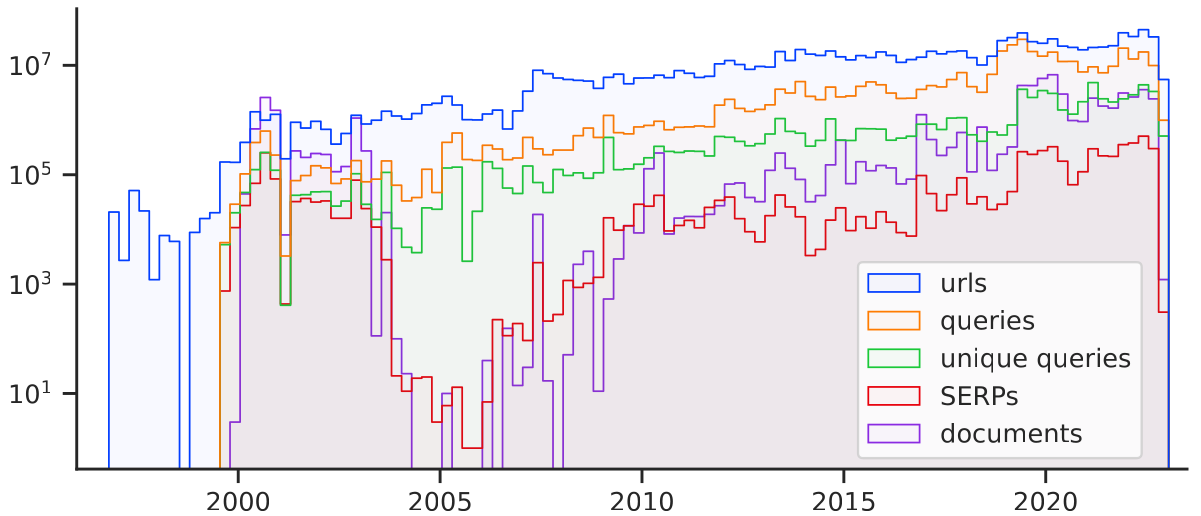
\includegraphics[width=\linewidth]{time-coverage}
    \end{column}
  \end{columns}
  \uncover<2->{
    \begin{block}{And now?}  
      \vspace{1ex}
      \begin{itemize}
        \item high diversity: topic and language
        \item diachronic analyses
        \item publically accessible via \href{https://www.tira.io/task/archive-query-log}{TIRA}
      \end{itemize}
    \end{block}  
  }
  \uncover<3>{\thankyou}
\end{frame}

% \appendix
% \bibliographyframe

\end{document}